\subsection{Magnetohydrodynamic shock wave}
In the magnetohydrodynamic case the same initial conditions where used, but a uniform magnetic field in the $x$-direction was added. The simulation was done for varying strengths of the magnetic field.
In \autoref{fig:MHD-blasts} a snapshot of the blast wave after 1 unit of time is plotted for different values of $\beta$.

\begin{figure}[H]
	%\hspace{-1cm}
	\centering
	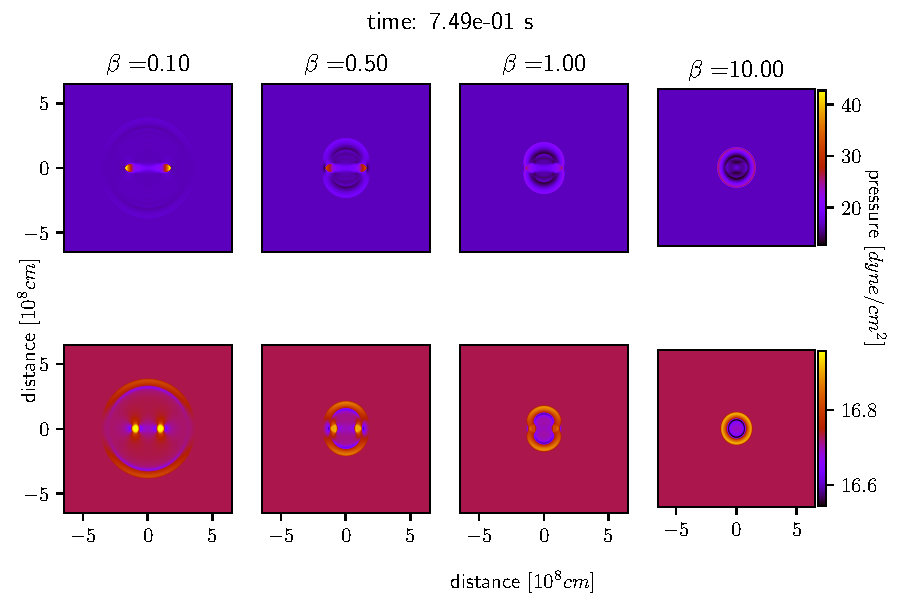
\includegraphics[width=\linewidth]{images/MHD-blasts.pdf}
	\caption{Plots of the pressure of an MHD blastwave with the same intial conditions as in \autoref{fig:HD-blast-short}: high pressure difference for the top row, lower for the bottom row.}
	\label{fig:MHD-blasts}
\end{figure}
in the plots with $\beta \in \{0.5,1\}$ there is a clear distinction between a fast shock wave spreading in all directions, and two small waves following the magnetic field.
In the plot with $\beta=0.1$ this fast wave is barely visible nearing the edge of the domain, but the two small waves stand out from the uniform background.
for $\beta=1$ the fast wave is almost perfectly spherical and very visible, while the two smaller waves are very faint.
We observe that if the magnetic field gets stronger, the wave becomes faster and most of the energy gets concentrated in the slow-mode, while the fast mode gets less energetyic. \improvement{calculate this flux?}
To go a bit more in-depth we plot the diagram depiciting the group speeds over the simulation data and see how well they match. This can be seen in \autoref{fig:MHD-group1} and \autoref{fig:MHD-group2}.

Since the initial condition is not a delta function, the wave will not nicely lie on the diagram of the group speed.
We have to correct for the finite radius of the circle with higher pressure in the initial condition.
By adding this circle to the diagram of the group speed, where the relevant speeds $v_a$, $v_s$ to calculate the group speed are found using \autoref{eq:Alfven-code-units} and \autoref{eq:sound-code-units}, the dashed lines are found.
These dashed lines do form an acurate boundary of the waves.
However for the fast wave mode we can make the same remark as in the hydrodynamic case: namely that the wave is faster then the linear wave in a medium with pressure $p_0$ due to the shock at the start.

We also see again that the wave is faster with a highr pressure difference. 
Due to the difficulty of accurately detecting the waves in the simulation data, either because they are realy faint with small or large $\beta$, or there is a lot of interference between the modes when $\beta \sim 1$, no accurate calculations of the wave speed from the simulation data could be made.

The effects of the magnetic field are clear, removing the isotropy of the wave and introducing two stron wave modes following the magentic field in oposite direction.
When the magnetic field becomes small, a quick comparison shows that the wave speed goes to the wave speed of an HD-wave as expected.

\begin{figure}[H]
	%\hspace{-1cm}
	\centering
	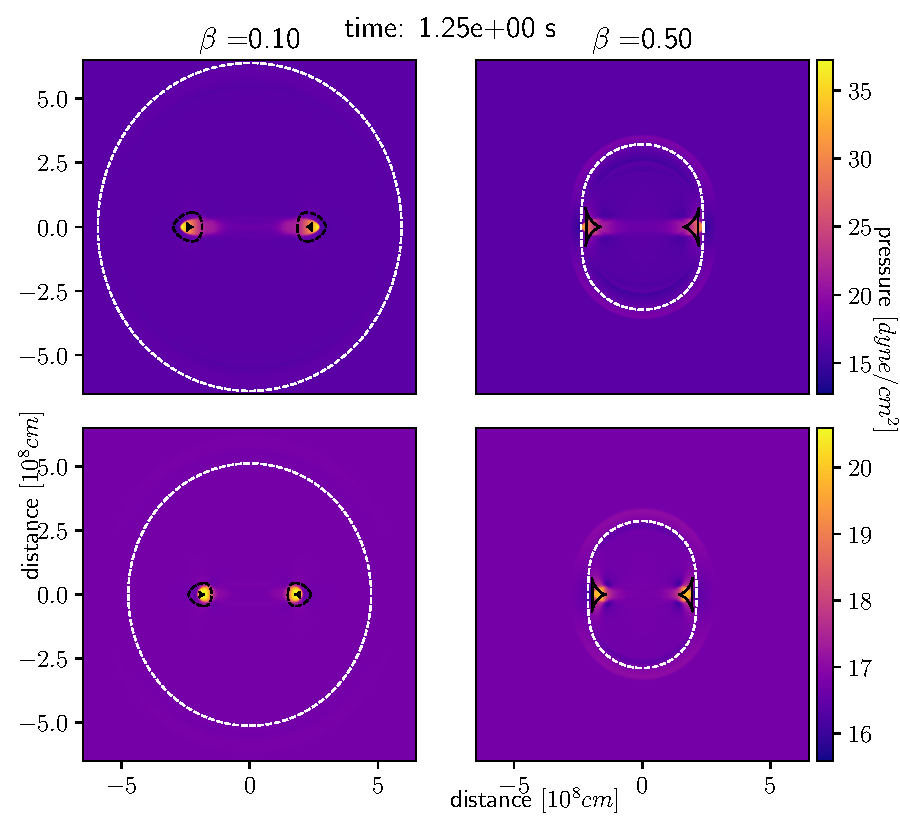
\includegraphics[width=\linewidth]{images/group-speed-pressure1.pdf}
	\caption{Plots of the pressure wave after $1.25$ time units for different values of $\beta$. The white dotted line represents the theoretical position of the fast mode magneto-accoustic wave. The black solid lines are the parts of the group speed diagram corresponding to the slow-mode magnetoaccoustic wave, and the black dotted lines are the is this privious curve "added" to the circle from the inital condition. This forms a boundary within which the slow mode wave propagates.}
	\label{fig:MHD-group1}
\end{figure}

\begin{figure}[H]
	%\hspace{-1cm}
	\centering
	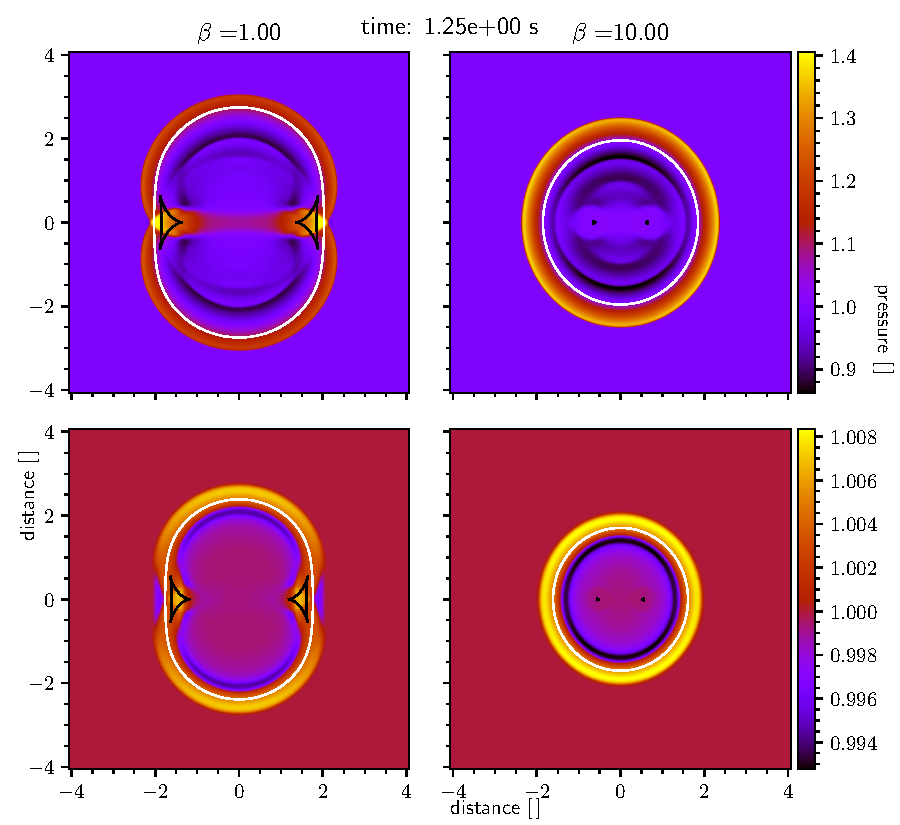
\includegraphics[width=\linewidth]{images/group-speed-pressure2.pdf}
	\caption{Same as \autoref{fig:MHD-group1} but for different $\beta$ values.}
	\label{fig:MHD-group2}
\end{figure}


